\documentclass[12pt,a4paper]{article}

%\usepackage[left=1.5cm,right=1.5cm,top=1cm,bottom=2cm]{geometry}
%\usepackage[in, plain]{fullpage}
\usepackage{array}
%\usepackage{../../../pas-math}
\usepackage{../../../moncours2}





%\makeatletter
%\renewcommand*{\@seccntformat}[1]{\csname the#1\endcsname\hspace{0.1cm}}
%\makeatother


%\author{Olivier FINOT}
\date{}
\title{}

%\newcommand{\disp}{false}

%
%\rfoot{Page \thepage}
\begin{document}
%\maketitle

\begin{myact}{1 Différentes écritures des nombres}
	
	\label{act:nbres}
	
	\begin{enumerate}
		\item Donner deux nombres à 2, 3, 4 et 5 chiffres.
		
		%\item \'Ecrire les nombres suivants en toutes lettres : \num{32}, \num{128} et \num{1024}. 
		\item \'Ecrire  le nombre 25146041337 en séparant les classes.
		\item La planète Mars a un rayon d'environ \textbf{3,4 milliers} de km, une superficie d'environ \textbf{144,8 millions} de $km^2$ et un volume d'environ \textbf{163 milliards} de $km^3$.
		
		\'Ecrire les trois nombres en gras en utilisant que des chiffres.
		
		\item Lire le texte ci-dessous, puis écrire en chiffres les nombres en gras.
		
		\begin{center}
			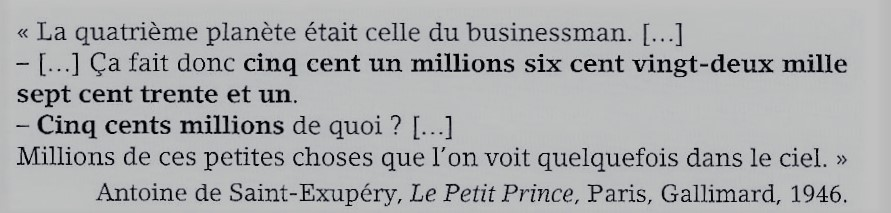
\includegraphics[scale=1.1]{img/act1}
		\end{center}
	\end{enumerate}
\end{myact}
%
\vspace*{2cm}

\begin{myact}{1 Différentes écritures des nombres}
	
	\label{act:nbres}
	
	\begin{enumerate}
		\item Donner deux nombres à 2, 3, 4 et 5 chiffres.
		
		%\item \'Ecrire les nombres suivants en toutes lettres : \num{32}, \num{128} et \num{1024}. 
		\item \'Ecrire  le nombre 25146041337 en séparant les classes.
		\item La planète Mars a un rayon d'environ \textbf{3,4 milliers} de km, une superficie d'environ \textbf{144,8 millions} de $km^2$ et un volume d'environ \textbf{163 milliards} de $km^3$.
		
		\'Ecrire les trois nombres en gras en utilisant que des chiffres.
		
		\item Lire le texte ci-dessous, puis écrire en chiffres les nombres en gras.
		
		\begin{center}
			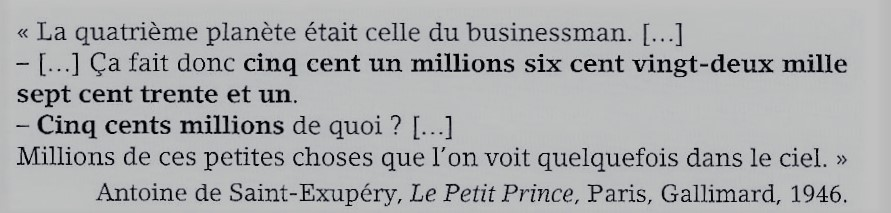
\includegraphics[scale=1.1]{img/act1}
		\end{center}
	\end{enumerate}
\end{myact}
%
%
%\begin{center}
%	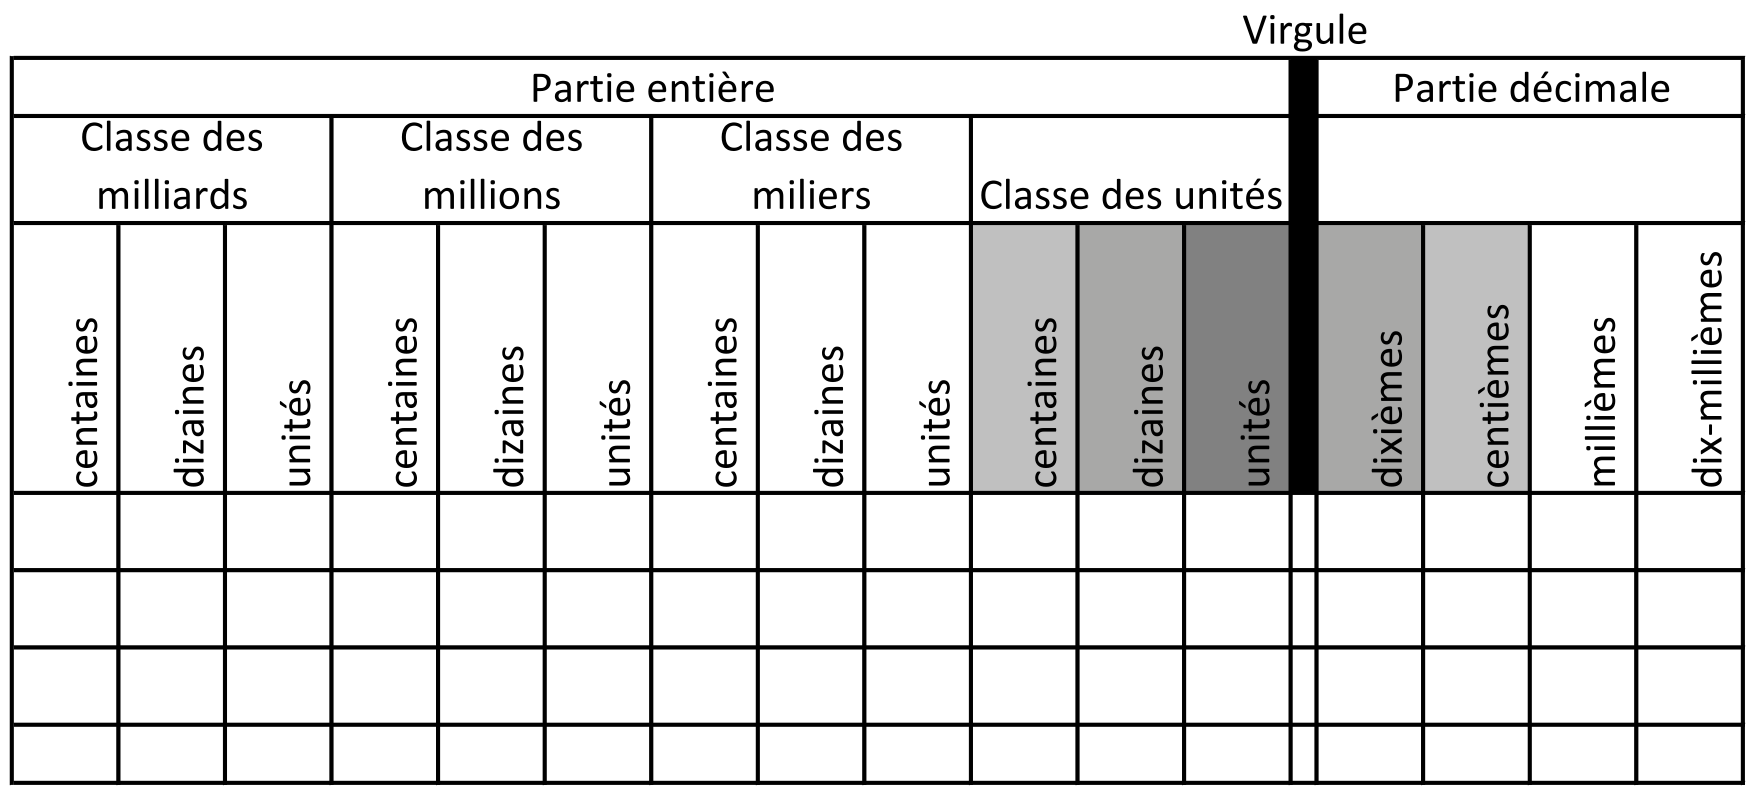
\includegraphics[scale=0.3]{img/tab_rangs}
%\end{center}
%
%\vspace*{0.5cm}
%\begin{center}
%	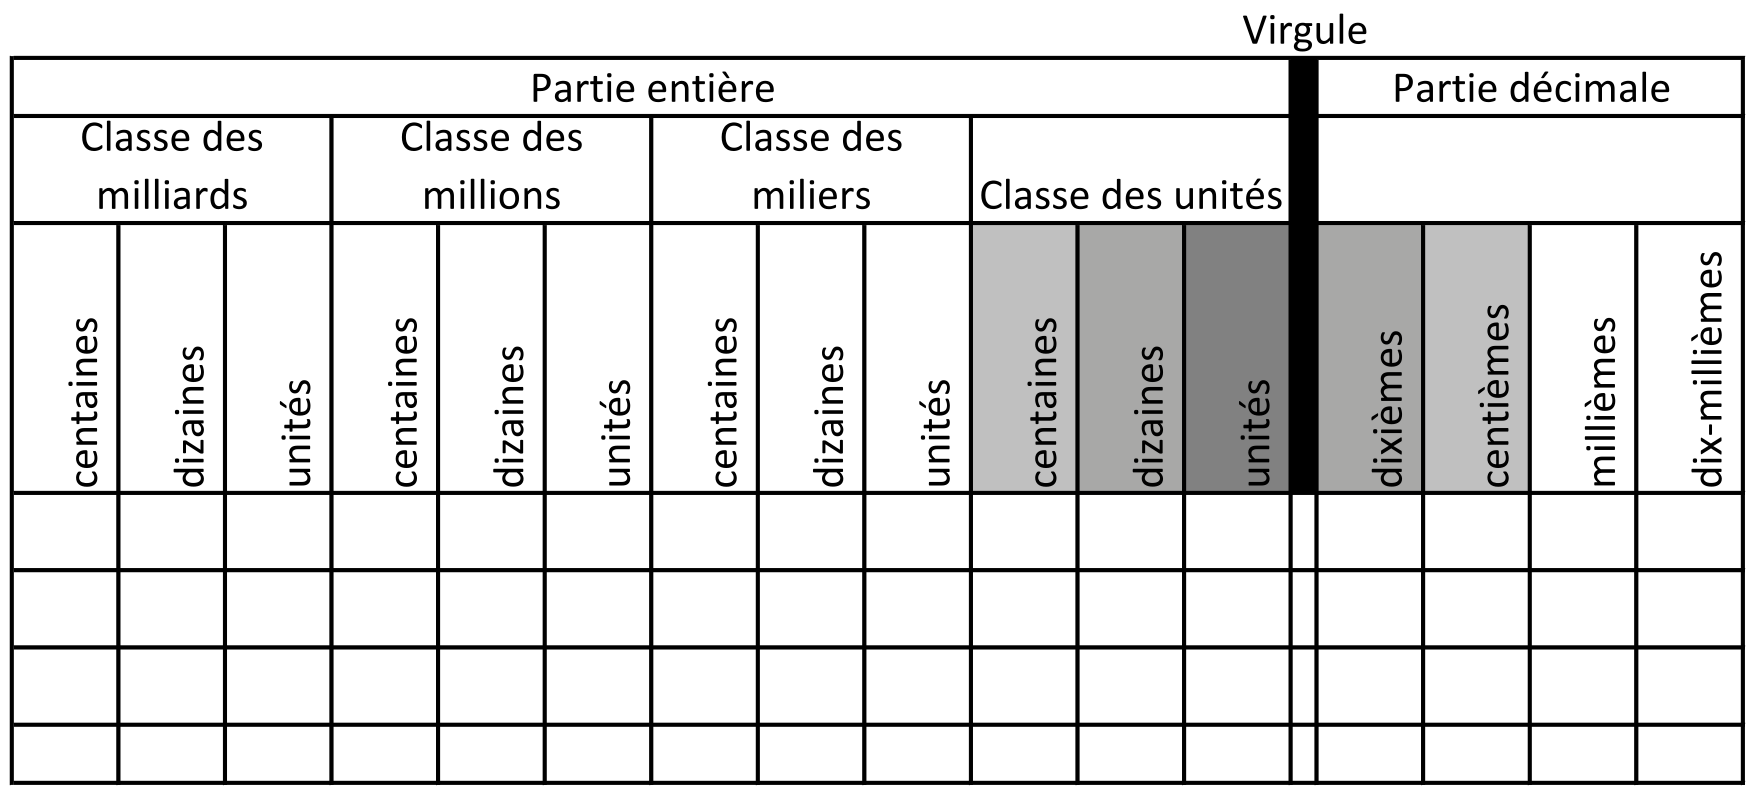
\includegraphics[scale=0.3]{img/tab_rangs}
%\end{center}
%
%\vspace*{0.5cm}
%
%\begin{center}
%	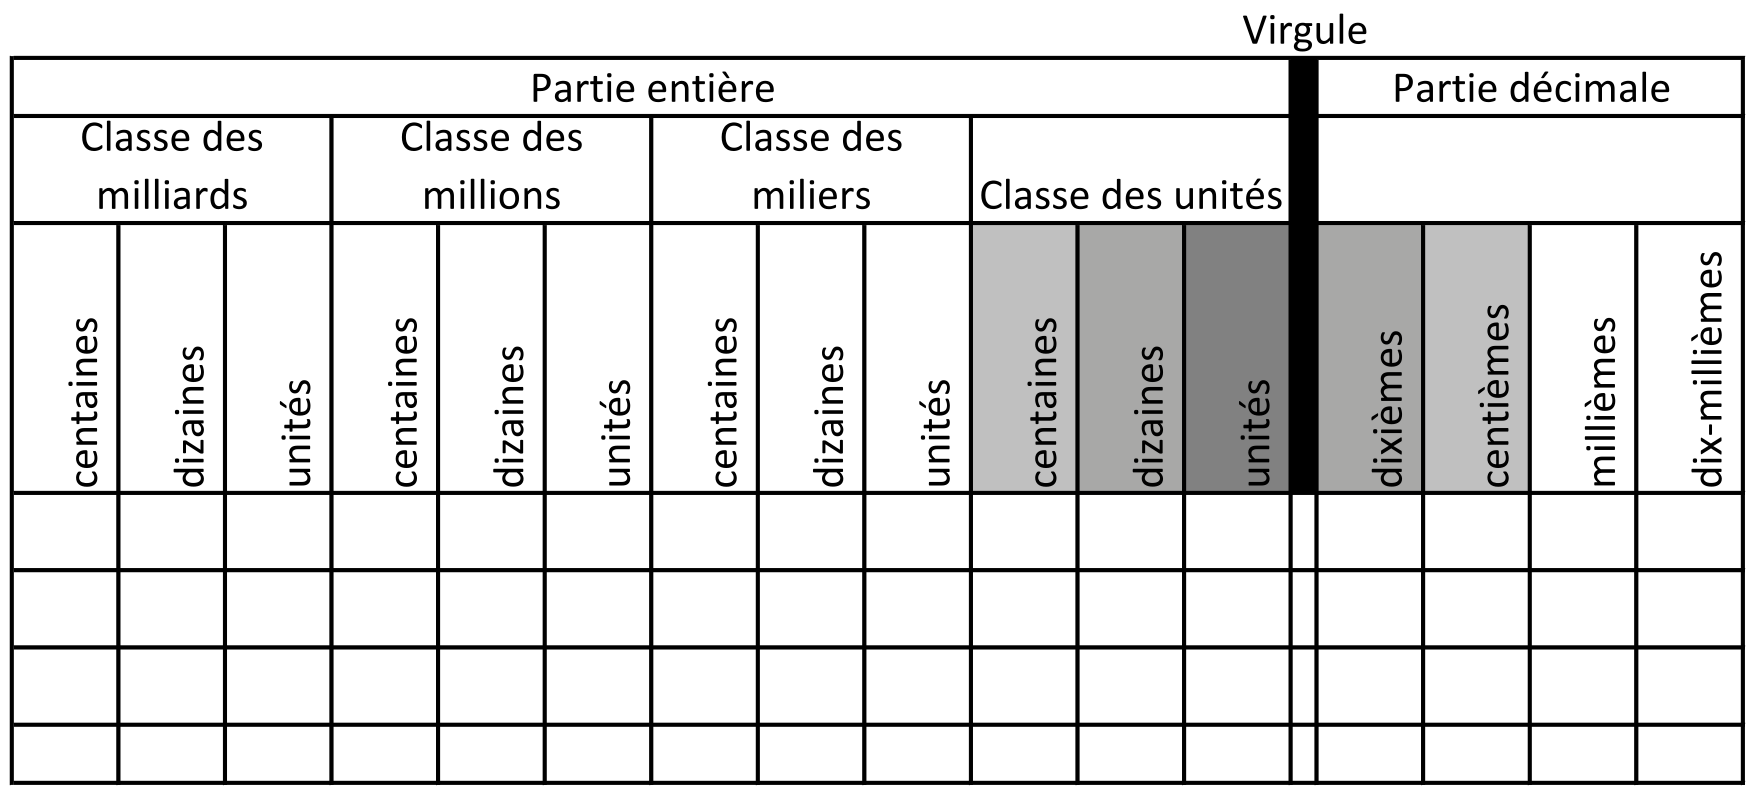
\includegraphics[scale=0.3]{img/tab_rangs}
%\end{center}


%\begin{myex}
%	\begin{center}
%		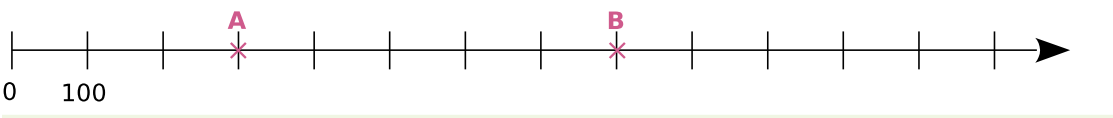
\includegraphics[scale=0.5]{img/axe}
%	\end{center}
%	
%	\begin{itemize}
%		\item L'abscisse du point A est :
%		\item L'abscisse du point B est :
%		\item L'abscisse du point C est : 500;
%		\item L'abscisse du point D est \num{1100}.
%	\end{itemize}
%\end{myex}
%
%\begin{myex}
%	\begin{center}
%		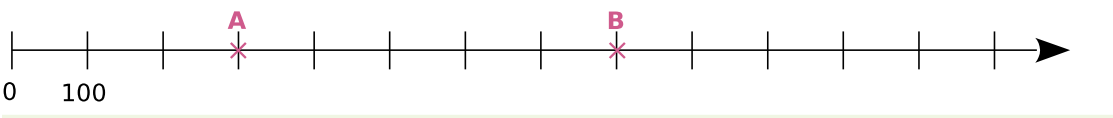
\includegraphics[scale=0.5]{img/axe}
%	\end{center}
%	
%	\begin{itemize}
%		\item L'abscisse du point A est :
%		\item L'abscisse du point B est :
%		\item L'abscisse du point C est : 500;
%		\item L'abscisse du point D est \num{1100}.
%	\end{itemize}
%\end{myex}
%
%\begin{myex}
%	\begin{center}
%		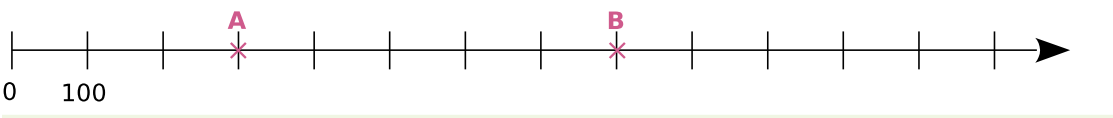
\includegraphics[scale=0.5]{img/axe}
%	\end{center}
%	
%	\begin{itemize}
%		\item L'abscisse du point A est :
%		\item L'abscisse du point B est :
%		\item L'abscisse du point C est : 500;
%		\item L'abscisse du point D est \num{1100}.
%	\end{itemize}
%\end{myex}
%



	
\end{document}